\documentclass[11pt]{standalone}

\usepackage{lmodern}	% font definition
\usepackage{amsmath}	% math fonts
\usepackage{amsthm}
\usepackage{amsfonts}
\usepackage{pgfplots}

\usepackage{pgfplots}
\usepackage{xcolor}
\usetikzlibrary{positioning,bayesnet}
\definecolor{brinkpink}{rgb}{0.98, 0.38, 0.5}
\definecolor{aogreen}{rgb}{0.0, 0.5, 0.0}
\usepackage{tikz}
\usetikzlibrary{decorations.pathmorphing} % noisy shapes
\usetikzlibrary{fit}					% fitting shapes to coordinates
\usetikzlibrary{backgrounds}	% drawing the background after the foreground
\pgfplotsset{compat=newest}% <-- moves axis labels near ticklabels (respects tick label widths)

\begin{document}
  \pgfplotsset{every tick label/.append style={font=\normalsize}}
  \pgfplotsset{every axis label/.append style={font=\normalsize}}
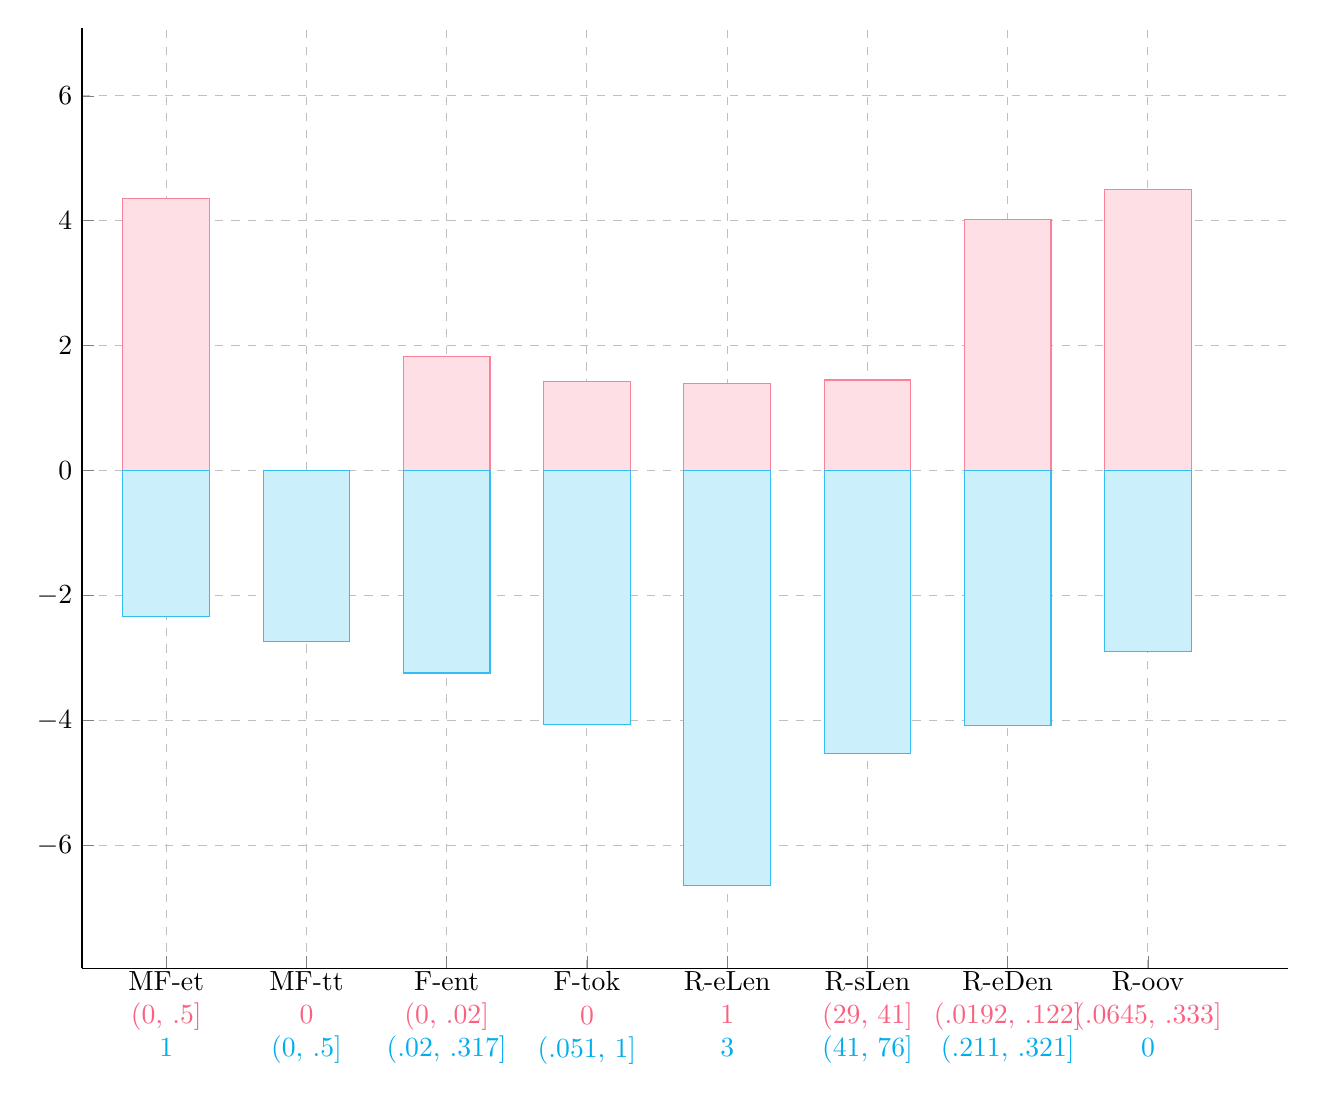
\begin{tikzpicture}
  \centering
  \begin{axis}[%ybar=1.0pt,
    ybar stacked,
    height=13.52cm,
    %width=16.9cm, % 12->9,  9->6.93,  8-> 6
    width=16.9cm, % 12->9,  9->6.93,  8-> 6
    bar width=1.1cm,
    xmin=0.4,
    xmax=9,
    ymin=-7.968,
    ymax=5.118888888888889,
    enlarge y limits={upper,value=0.15},
    axis lines*=left,
    legend style={at={(0.5,-0.25)},anchor=north,legend columns=-1,
    /tikz/every even column/.append style={column sep=0.2cm}},
    %xticklabels={\textcolor{brinkpink}{S}-\textcolor{aogreen}{L},\textcolor{brinkpink}{M}-\textcolor{aogreen}{S},\textcolor{brinkpink}{L}-\textcolor{aogreen}{M},\textcolor{brinkpink}{S}-\textcolor{aogreen}{S},\textcolor{brinkpink}{M}-\textcolor{aogreen}{M},\textcolor{brinkpink}{L}-\textcolor{aogreen}{L},\textcolor{brinkpink}{S}-\textcolor{aogreen}{S},\textcolor{brinkpink}{M}-\textcolor{aogreen}{M}},
    xticklabels={MF-et \\ \textcolor{brinkpink}{(0, .5]} \\ \textcolor{cyan}{1}, MF-tt \\ \textcolor{brinkpink}{0} \\ \textcolor{cyan}{(0, .5]}, F-ent \\ \textcolor{brinkpink}{(0, .02]} \\ \textcolor{cyan}{(.02, .317]}, F-tok \\ \textcolor{brinkpink}{0} \\ \textcolor{cyan}{(.051, 1]}, R-eLen \\ \textcolor{brinkpink}{1} \\ \textcolor{cyan}{3}, R-sLen \\ \textcolor{brinkpink}{(29, 41]} \\ \textcolor{cyan}{(41, 76]}, R-eDen \\ \textcolor{brinkpink}{(.0192, .122]} \\ \textcolor{cyan}{(.211, .321]}, R-oov \\ \textcolor{brinkpink}{(.0645, .333]} \\ \textcolor{cyan}{0}},
    xtick=data,
    xmajorgrids=true,
    ymajorgrids=true,
    zmajorgrids=true,
    grid style=dashed,
    xticklabel style={
        inner sep=1pt,
	align=center,
        %rotate=90,
        %anchor=near xticklabel,
    },
    ]
    %\addplot [draw=aogreen!80,fill=aogreen!20] table[x=id,y=y]{
    \addplot [draw=cyan!80,fill=cyan!20] table[x=id,y=y]{
    id  y
    	1	-2.34
	2	-2.73
	3	-3.24
	4	-4.07
	5	-6.64
	6	-4.53
	7	-4.08
	8	-2.9
    };
    \addplot [draw=brinkpink!80,fill=brinkpink!20] table[x=id,y=y]{
    id  y
    	1	4.36
	2	0.0
	3	1.82
	4	1.42
	5	1.4
	6	1.45
	7	4.02
	8	4.5
    };
  \end{axis}
\end{tikzpicture}

\end{document}

